%%%%%%%%%%%%%%%%%%%%%%%%%%%%%%%%%%%%%%%%%%%%%%%%%%%%%%%%%%%%%%%%%%%%%%%%%%%%%%%%

\documentclass{article}
\usepackage{amssymb, amsmath, graphicx, enumerate, mathtools, listings, algorithm, algpseudocode}

\setlength{\oddsidemargin}{.25in}
\setlength{\evensidemargin}{.25in}
\setlength{\textwidth}{6in}
\setlength{\topmargin}{-0.4in}
\setlength{\textheight}{8.5in}

%%%%%%%%%%%%%%%%%%%%%%%%%%%%%%%%%%%%%%%%%%%%%%%%%%%%%%%%%%%%%%%%%%%%%%%%%%%%%%%%
% PACKAGES
%
\usepackage{fullpage}
\usepackage[pdftex]{hyperref}
\usepackage{amsthm}
\usepackage[draft]{todonotes}
\usepackage{times}
\usepackage{comment}
\usepackage{xspace}
\usepackage{paralist}
\usepackage{enumitem}
  \setlist[itemize]{leftmargin=*}
  \setlist[enumerate]{leftmargin=*}
\usepackage{makecell}
\usepackage{tikz}
	\usetikzlibrary{matrix,shapes,arrows,positioning,chains,calc}
\usepackage{hypcap}
\usepackage{mleftright}
\usepackage{bbm}
\usepackage{colortbl}
\usepackage{tabu}
\usepackage{multirow}
\usepackage{mathrsfs}
\usepackage{adjustbox}
\usepackage{microtype}
\usepackage{etoolbox}
\usepackage{breakcites}
\usepackage{booktabs}
\usepackage[framemethod=tikz]{mdframed}
\usepackage{soul}
\usepackage[small,margin=2mm]{caption}
\usepackage{subcaption}
\usepackage{float}
\usepackage{iitem}
\usepackage{scalerel}
\usepackage{rotating}
\usepackage{verbatimbox}
\usepackage{complexity}
\usepackage{mathtools}
\usepackage{braket}
\usepackage{relsize}
\usepackage{extarrows}
\usepackage{graphicx}
\usepackage{csquotes}
\usepackage{hyperref}
\usepackage[backend=biber,style=alphabetic,sorting=anyt]{biblatex}
\bibliography{zk-SNARKs}
\renewcommand*{\bibfont}{\small}
%%%%%%%%%%%%%%%%%%%%%%%%%%%%%%%%%%%%%%%%%%%%%%%%%%%%%%%%%%%%%%%%%%%%%%%%%%%%%%%%
%%%%%%%%%%%%%%%%%%%%%%%%%%%%%%%%%%%%%%%%%%%%%%%%%%%%%%%%%%%%%%%%%%%%%%%%%%%%%%%%

%%%%%%%%%%%%%%%%%%%%%%%%%%%%%%%%%%%%%%%%%%%%%%%%%%%%%%%%%%%%%%%%%%%%%%%%%%%%%%%%
% THEOREM ENVIRONMENTS
\newtheorem{theorem}{Theorem}%[section]
\newtheorem{corollary}{Corollary}[section]
\newtheorem{proposition}[corollary]{Proposition}
\newtheorem{definition}[corollary]{Definition}
\newtheorem{lemma}[corollary]{Lemma}
\newtheorem{claim}[corollary]{Claim}
\newtheorem{observation}[corollary]{Observation}
\newtheorem{notation}[corollary]{Notation}
\newtheorem{fact}[corollary]{Fact}
\newtheorem{assumption}[corollary]{Assumption}
\newtheorem{conjecture}[corollary]{Conjecture}
\newtheorem{goal}[corollary]{Goal}
\newtheorem{remark}[corollary]{Remark}
\newtheorem{question}[corollary]{Question}
\newtheorem{problem}[corollary]{Problem}
\newtheorem{challenge}[corollary]{Challenge}
\newtheorem{example}[corollary]{Example}
\newtheorem{exercise}[corollary]{Exercise}
%%%%%%%%%%%%%%%%%%%%%%%%%%%%%%%%%%%%%%%%%%%%%%%%%%%%%%%%%%%%%%%%%%%%%%%%%%%%%%%%

%%%%%%%%%%%%%%%%%%%%%%%%%%%%%%%%%%%%%%%%%%%%%%%%%%%%%%%%%%%%%%%%%%%%%%%%%%%%%%%%
% MACROS

%-----------------------------------------------------------------------------
% Special-purpose color definitions (dark enough to print OK in black and white)
\usepackage{color}

% A few colors to replace the defaults for certain link types
\definecolor{orange}{cmyk}{0,0.4,0.8,0.2}
\definecolor{darkorange}{rgb}{.71,0.21,0.01}
\definecolor{darkgreen}{rgb}{.12,.54,.11}

%-----------------------------------------------------------------------------
% The hyperref package gives us a pdf with properly built
% internal navigation ('pdf bookmarks' for the table of contents,
% internal cross-reference links, web links for URLs, etc.)

\hypersetup{  % needed for pdflatex
  breaklinks=true,  % so long urls are correctly broken across lines
  colorlinks=true,
  urlcolor=blue,
  linkcolor=darkorange,
  citecolor=darkgreen,
}

%-----------------------------------------------------------------------------
\newcommand{\N}{{\mathbf N}}
\newcommand{\Z}{{\mathbf Z}}
\newcommand{\F}{{\mathbf F}}
\newcommand{\Q}{{\mathbf Q}}
\newcommand{\Time}{\operatorname{time}}
\newcommand{\negl}{\mathsf{negl}}
\newcommand{\ci}{\stackrel{c}{=}}
\newcommand{\si}{\stackrel{\Delta}{=}}
\newcommand{\io}{i\mathcal{O}}
\newcommand{\scheck}{\textbf{\textit{\textcolor{red}{Sanity Check: }}}}

\mdfsetup{
    roundcorner=10pt,
    frametitlebackgroundcolor=cyan!15!green!15,
    backgroundcolor=cyan!15!green!15,
    hidealllines=true,
    skipabove=12pt,
    skipbelow=6pt,
    leftmargin=0pt
    rightmargin=0pt,
    innertopmargin=-4pt,
    innerbottommargin=8pt,
    innerleftmargin=12pt,
    % innerrightmargin=12pt,
    % frametitleaboveskip=6pt,
    % frametitlebelowskip=4pt,
    % frametitlerule=true,
    % frametitlefont=\normalfont\itshape,
    splittopskip=2\topsep
}

\pagenumbering{gobble}
\title{zk-SNARKs}
\author{Alex Kazorian}
\date{\today}
\graphicspath{ {/} }

\begin{document}
\maketitle
\section*{Introduction}
Whether or not we are in a cryptocurrency bubble is not what drives the discussion of zk-SNARKs. Yes, zcash is the currency that introduced many people to the topic of this write up; however, the effect of zk-SNARKs could be wider reaching than a cryptocurrency. \\ \\
\noindent This article will be broken up into three parts, each meant to explain the topic to a seperate audience. These audiences are the average adult, an undergraduate focusing on computer science or math, and a graduate student interested in cryptography or some complexity theoritic topic or another. Below is a dependency graph to help in navigating the sections in this article. Note that the dotted line indicates that section two is a "soft prerequisite" for understanding section 3. This is because section 3 assumes graduate level maturity. If you are not comfortable with the material in this section, try revisiting it after reading section 2.
\begin{center}
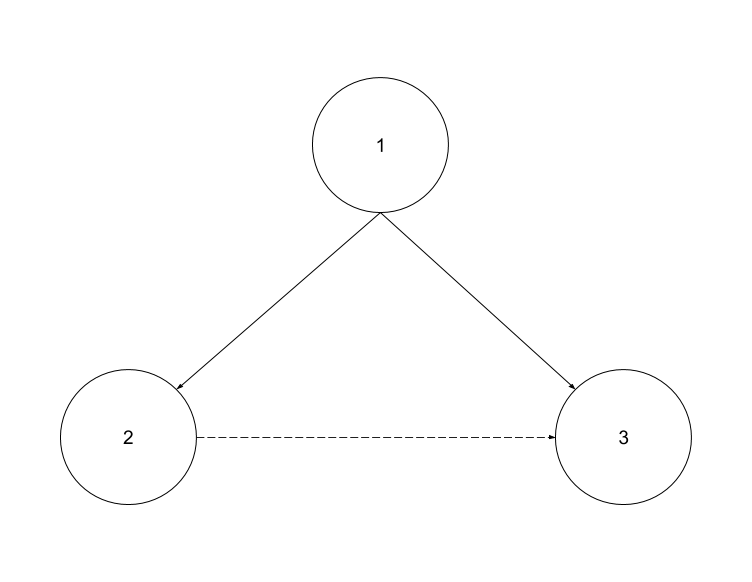
\includegraphics[scale=0.4]{zk-SNARK_fig1}
\end{center}
For all three audiences, it will be benefitial to know what zk-SNARK is an acronym of. Yeah it's a catchy thing to say, but it is quite descriptive of an acronym. A zk-SNARK is a zero-knowledge, Succinct, Non-interactive, ARgument of Knowledge and that really is a mouthfull.

\subsection*{Motivation}
When trying to understand a cryptographic primitive it always helps to understand why it exists. In other words, what problem does it solve? In doing so, we will have the necessary motivation to drive future research and curiosity! Let's get to it by first introducing our main characters Alice and Bob. Picture this: our protaganists reside in a dystopian society in the near future where government surveillance runs rampant. Alice and Bob are attempting to orchestrate a rebellion right under the nose of the black suits in office. They have found a hide out to base their operation from, but need a method of proving that a member knows the secret word for getting in. Moreover, no one should be able to learn the secret word or how to find it even if a third party person was listening in.


\section*{1. ELI5: A Primer For The Average Person}
The above scenario is admittedly very contrived; however, the above can be reworded into the following problem: how can we prove the integrity of encrypted data? zk-SNARKS are the solution to this problem. To answer why, we first delve into understanding the notion of a proof and knowledge.
\subsection*{1.1. What Is A Proof?}
As humans, we prove statements every day. We do so without even considering what the definition of a proof is and so let us slow down to consider a proof of a mathematical statement. Such proofs have the following properties:
\begin{enumerate}
    \item They consist of a static sequence of statements that follow in some logical order. These statements are therefore either axioms of mathematics or are derivational rules.
    \item The proof itself is at least as important as the theorem it is proving.
\end{enumerate}
Now, this type of proof would not help us in answering our question of proving integrity over encrypted data. Why? Once the proof is read out loud, it is trivially replicable and recitable. Therefore, a third party can trick us of say their identity as a fellow rebel. Looking ahead at the solution, one aspect of mathematical proofs remains. There are two parties present in such a proof system: the Prover and the Verifier.
\subsection*{1.2. What Is Knowledge?}
I'm no philosopher. Pass!
\subsection*{1.3. What Does It Mean To Gain Knowledge?}
Informally, one gains no knowledge from an interaction if and only if said person does not receive the proof for something that was otherwise infeasible for them to find themselves. For example, if someone told me that $1 + 1 = 2$, then I have gained no knowledge because I can do at least that much arithmetic. If, however, someone were to show me a proof of extraterrestial life forms, then I have certainly gained some knowledge.
\subsection*{1.4. Bringing It All Together}
We now possess the necessary intuition to derive an informal definition of a zk-SNARK. Recall that we know the following:
\begin{itemize}
    \item We want to derive a protocol that can allow for proving knowledge of a secret without anyone learning the proof itself.
    \item A proof requires a prover and a verifier.
    \item Without receiving the proof of something I otherwise could not have proved, I have learned nothing.
\end{itemize}
With this information, we outline the following properties necessary for a protocol that solves our problem:
\begin{itemize}
    \item \textit{Zero-knowledge:} The verifier gains no knowledge from the prover. In effect, the verifier does not learn the prover's proof and cannot use it later. This falls in line with our discussion regarding gaining knowledge.
    \item \textit{Succinct:} The verifier does not have listen to the prover for too long of a time. This does not mean that the prover cannot think for themselves before speaking to the verifier. It simply means the prover's response must be "small".
    \item \textit{Non-interactive:} The verifier and prover are not engaged in a "back-and-forth" conversation.
    \item \textit{ARgument of Knowledge:} The prover is able to show that they have knowledge of something. In our case, it would be the secret word.
\end{itemize}

\section*{2. Diving Deeper: zk-SNARKS for the curious}
We all ideally understand zk-SNARKs at the level of an average person, but we'll be formalizing the above notions for those of us who remain curious. I want to be very clear that the definition outlined in this section is \textbf{not} complete and is ignoring some very small technical details that are integral to the study of zk-SNARKs. The decision to omit these details is, in my opinion, necessary to able to discuss this primitive at the level of an undergraduate in Computer Science or mathematics without explaining everything taught in a graduate cryptography course. With that out of the way, let's brush up on some necessary background material!
\subsection*{2.1. Prerequisites}
\textbf{Note:} I will be assuming knowledge of \href{https://en.wikipedia.org/wiki/Asymptotic_analysis}{asymptotic analysis} and the level of mathematical maturity after having taken a discrete mathematics course.

\subsubsection*{2.1.1. \textsc{P} and \textsc{NP}}
\textbf{Definition:} \textit{The complexity class \textsc{P} is the set of all problems $\mathcal{P}$ that can be solved in polynomial time.} \\ \\
\textbf{Definition:} \textit{The complexity class \textsc{NP} is the set of all problems $\mathcal{P}$ that can be verified in polynomial time when given a potential solution $\pi$ to an instance of the problem $x$. Here $\pi$ acts as a proof of sorts for the membership of $x$ in the set of inputs with a solution for $\mathcal{P}$.} \\ \\
\noindent \textit{Remark:} Given these defintions, we know that \textsc{P} $\subseteq$ \textsc{NP}. Why is this the case? If we could find the solution to a problem, then of course we could verify the validity of any solution to said problem! However, the literal million dollar question is does \href{https://en.wikipedia.org/wiki/P_versus_NP_problem}{\textsc{P} $=$ \textsc{NP}?}

\subsubsection*{2.1.2. Algorithms and Randomness}
We later define our prover and verifier in terms of an algorithm and so we need to introduce some notation. An algorithm is said to accept its input if it outputs one after halting. On the other hand, if an algorithm outputs 0, then we say it rejected its input. Lastly, an important class of algorithms to consider are probabilistic polynomial time algorithms. These are algorithms that terminate in a polynomial number of steps but are allowed some randomness. This randomness is expressed through an algorithms ability to flip coins. Therefore, the probability of an event occuring related to a probabilistic polynomial time algorithm is always over the random coin tosses said algorithm has access to.

\subsubsection*{2.1.3. Negligible Functions}
A negligible function is something that is thrown around \textit{all the time} in the cryptographic literature. It is absolutely essential to know what functions are negligible. We should all be asking why are negligible functions used so often? The answer lies in the necessity to capture the notion of certain events being so unlikely that we need not consider them. Such events include breaking the security of algorithms which we discuss in the section regarding indistinguishability. \\ \\
\noindent An intuitive explanation of an event being unlikely is something like a function being exponentially small. In other words a function is small if it grows slower than \textit{every} polynomial function. This is a definition that we decided on because it satisfies our needs.\\ \\
\noindent \textbf{Definition:} \emph{A function $\mu$ is negligible if and only if $\forall{c} \in \N$, $\exists n_0 \in \N$ such that $\forall n \geq n_0$ it is the case that $\mu(n) < n^{-c}$.}

\subsubsection*{2.1.4. Indistinguishability}
Cryptography would be useless if we cannot guarantee the security of our primitives when under attack by adversaries. Most cryptographic primitives (if not all) are randomized algorithms. In effect, they are allowed to flip some number of coins during their execution. Because our primitives are randomized algorithms, they output a random variable with some distribution. Ideally, this random variable would distributed uniformally. \\ \\
\noindent \textbf{\textit{\textcolor{red}{Sanity Check:}}} Why would we want the distribution of the random variable outputted by some cryptographic primitive to be distributed uniformally? \\ \\
\noindent There are three notions of indistinguishability and they are in order of decreasing strength: perfect, statistical, and computational. \\ \\
\noindent \textbf{Definition:} \textit{A random variable $X$ is perfectly indistinguishable from the uniform distribution $U$ if the distribution of $X$ is equivalent to $U$. The notation used for this is $X \equiv U$ or $X \stackrel{p}{=} U$.} \\ \\
\noindent \textbf{Definition:} \textit{A random variable $X$ is statistically indistinguishable from the uniform distribution $U$ if the \href{https://en.wikipedia.org/wiki/Total_variation_distance_of_probability_measures}{total variation distance between} $X$ and $U$ is negligible. Intuitivally, this is an information theoretic argument saying that there does not exist a function or algorithm that can pull these two distributions any further apart. The notation used for this is $X \si U$.} \\ \\
\noindent \textbf{Definition:} \textit{A random variable $X$ is computationally indistinguishable from the uniform distribution $U$ if for every probabilistic polynomial time algorithm $A$ and for all security parameter $k \in \N$:}
$$\bigg\lvert \Pr[D(X) = 1] - \Pr[D(U) = 1]\bigg\rvert = \text{ negl}(k)$$
\textit{The notation used for this is $X \ci U$.}

\subsubsection*{2.1.5. Proof Systems}
Recall that a proof involves a prover and a verifier. Therefore, we have the following definition of a a proof system: \\ \\
\textbf{Definition:} \textit{A proof system is a pair of algorithms $(P, V)$ for a problem $\mathcal{P}$ such that below properties are satisfied:}
    \begin{enumerate}
        \item \textit{Efficiency: The verifier must run in polynomial time and is allowed access to some randomness.}
        \item \textit{Completeness: If the prover has a correct proof for the validity of a statement related to an instance of the problem $\mathcal{P}$, then the verifier must be convinced:}
        $$\Pr\bigg[V(x, \pi) = 1 \Bigg\vert \pi = P(x)\bigg] \geq \frac{2}{3}$$
        \item \textit{Soundness: The verifier cannot be tricked by any prover $P^*$ into believing statements about instances to the problem with no valid solution:}
        $$\Pr\bigg[V(x, \pi) = 1 \Bigg\vert \pi = P^*(x)\bigg] \leq \frac{1}{3}$$
    \end{enumerate}
\noindent \textit{Remark:} We allow the verifier to fail with a probability of a third for completeness because we repeat the protocol for any proof system to drive down the probability of failure. A similar argument can be made for the error probability of the soundness property. \\ \\
\subsection*{2.2. Adding Some Formalities}
We are not too far from being able to have some formality when discussing the definition of a zk-SNARK. At this point, we only really have a basic proof system. We're missing quite a bit from our zk-SNARK acronym so let us dive right in!
\subsubsection*{2.2.1. Non-interactive Proof Systems}
Because I don't expect everyone to know what an interactive proof system is, the above definition for a proof system suffices for the level of understanding we are going for with zk-SNARKs in this section. Do note that the above definition is missing a detail that will be touched on extensively in the last section of this write up.
\subsubsection*{2.2.2. From Proof Systems to ARgument Systems}
Looking back at our property for efficiency of a proof system, its clear that I did not specify any requirements for the prover. This is because in many proof systems, we do not care about how long it takes for the prover to come up with the a proof. In real life, all I care about is if I am convinced. Yes, this is quite selfish but such is life. Instead, we want an efficient verification process; therefore, the majority of the work falls on the shoulders of the prover in a proof system. A prover is computationally unbounded often times for this very reason. Now, this is interesting. There is a clear discrepancy between the amount of work expected of the prover and the amount of work expected of the verifier, but this imbalance in power or efficiency should remind us of something––\textsc{NP}! The complexity class \textsc{NP} can be thought of a class for problems with a proof system. \\ \\
\noindent \textbf{\textit{\textcolor{red}{Sanity Check:}}} Can you define the complexity class \textsc{NP} in terms of a proof system? Don't be afraid to redefine soundness and completeness to satisfy \textit{your} needs. This is math and as mathematicians, we are the wizards! \\ \\
\noindent This is all great, but do we really have unlimited time for provers. Say you are able to verify something quickly. If the prover cannot supply me with a proof to verify before life on Earth ends, then what good is our proof system. There are reasons to consider proof systems for which the prover is computationally unbounded; however, we can relax our definition of a proof system by requiring that the prover is computationally bounded. One might ask: "how is this a relaxation of the problem?" Well our definition will now account for a set of provers that is less powerful. Therefore, possibly malicious provers are also less powerful and the above properties are easier to satisfy. We refer to this "relaxed" definition as a Computationally Sound Non-interactive Proof or a Non-interactive ARgument. Woohoo, we have NAR!
\subsubsection*{2.2.3. Succinctness}
The proofs the verifier receives should ideally be small. Why? A smaller proof that satisfies the above conditions for a NAR can only improve the efficiency of the verifier. So the question to ask is more along the lines of why wouldn't we want this? More formally, we add the following property to our NAR:

5. \textit{Succinctness: The size of the proof is polynomial in the size of the problem instance. In other words, for an instance $x$ of problem $\mathcal{P}$, $\pi = p(\lvert x \rvert)$ for some polynomial $p$ where $\pi$ is the output of $P(x)$.} \\ \\
\noindent The scoreboard has us at SNAR. What's left?

\subsubsection*{2.2.4. Zero-knowledge and the Simulation Paradigm}
Previously, we defined the property of zero-knowledge to be such that "the verifier does not learn the prover's proof and cannot use it later". We have some new tools in our tool belt and we will use them to formulate a definition that satisfies \textit{our} needs. First, what does it mean to "learn" a proof? I argue that this means the verifier is able to replicate the proof for any input with a satisfying solution to the problem our proof system is defined under. How can we guarantee this cannot happen? \\ \\
\noindent In a non-interactive proof system, the verifier sees only the proof $\pi$ and the input $x$. If the verifier learns nothing outside of these two from the protocol, then there is no way the verifier could have learned the proof. To formalize this notion, we introduce the idea of a simulator. A simulator $S$ is an algorithm that outputs a random variable. Because the output of the protocol between the prover and verifier is a random variable as well, we want the distribution of these random variables to be indistinguishable. The level of indistinguishability can vary meaning that our proof system can have perfect, statistical, or computational zero-knowledge. More formally, \\ \\
\noindent \textbf{Definition: } \textit{A proof system $(P, V)$ for a problem $\mathcal{P}$ is zero-knowledge if there exists a probabilistic polynomial time simulator $S$ such that for all $x$ with solutions to $\mathcal{P}$,}
$$\{x, P(x)\} \stackrel{p/\Delta/c}{=} S(x)$$
\\
\noindent \scheck I heavily relied on notational macros to shorten the definition. Rewrite the definition for the three different notions of zero-knowledge more explicitly. Once you have done this, we now have zk-SNARs. One more letter...

\subsubsection*{2.2.5. zk-SNAR of Knowledge}
Thus far, we have discussed proof systems for which a prover can prove whether or not a statement is true. Just as a reminder, the statements are asked by the verifier and are of the form "does $x$ have a solution to the problem $\mathcal{P}$". Therefore, with our current definitions, we can answer the question "is $x$ the secret word for entrance?" Really we want someone to prove why $x$ is the secret word for entrance. This is the idea behind a proof of knowledge. \\ \\
\noindent Now, we need to formulaize this notion of the prover "knowing a secret". Recall that the zero-knowledge property of the proof system we are working with is such that the prover is not going to just reveal their proofs of \textit{anything}. However, if a prover knows something, then we should be able to extract it. More formally, \\ \\
\noindent \textbf{Definition: } \textit{A proof system $(P, V)$ is a proof of knowledge if there exists a probabistic polynomial time extractor E such that for all provers $P^*$ and for all $k \in \N$ the following property of Extractability holds,}
$$\Pr\bigg[\begin{array}{c} (x, \pi) \leftarrow P^*(z) \\ V(x, \pi) = 1\end{array} \wedge \begin{array}{c} (x, w) \leftarrow E^{P^*}(z) \\ w \text{ is not a solution for } x \text{ under problem } \mathcal{P}\end{array}\bigg]$$
\\
\noindent \textit{Remark: } Here the proof $\pi$ is a proof of the statement "$w$ is a solution to $x$ for problem $\mathcal{P}$. Moreover, the funky notation for $E^{P^*}$ is saying that $E$ has "oracle" access to $P^*$. This means that $E$ can makes function calls to $P^*$.\\ \\
\noindent $<$Wipes sweat from forehead$>$ There. zk-SNARKs. Done.

\section*{3. The Real Thing: zk-SNARK}
Again, I assume graduate level maturity of complexity theory and cryptography. This really is an advanced primitive and requires a delicate treatment of the definitions of simpler primitives.

\subsection*{3.1. Prerequisites}

\subsubsection*{3.1.1. NP Relations}
\textbf{Definition:} \textit{A relation $R$ for some language $\mathcal{L}$ is the set of instance, witness pairs $(x, w)$ such that $\mathcal{L}_{R} := \{x : \exists w s.t (x, w) \in R\}$}.

\scheck Can you define the class of languages \textsc{NP}?

\textbf{Definition:} \textit{The universal relation $R_U$ is the set of instance, witness pairs $(x, w)$ where $x = (M, y, t)$. Here, $|x|, |w| \leq t$ and $M$ is a random access machine that accepts the input $(y, w)$ in $O(t)$ steps.}

\textit{Remark: } $R_U$ is the relation for the universal language $\mathcal{L}_U$.
\subsubsection*{3.1.2. Common Reference String Model}
In section 2, the definition of Non-interactive Proof Systems was said to be missing something. It's missing randomness. Think about it. A non-interactive proof system with no randomness is unidirectional and gives no leeway to have a zero-knowledge property. Why? The prover could only prove their statement
\end{document}
